\section{Sensational EM \hpoints{23}}

Suppose we have a robot with a single unreliable range sensor. For
example, if the robot is standing 3 meters away from the nearest
obstacle, we might get readings like this:
\begin{figure}[h!]
  \centering
  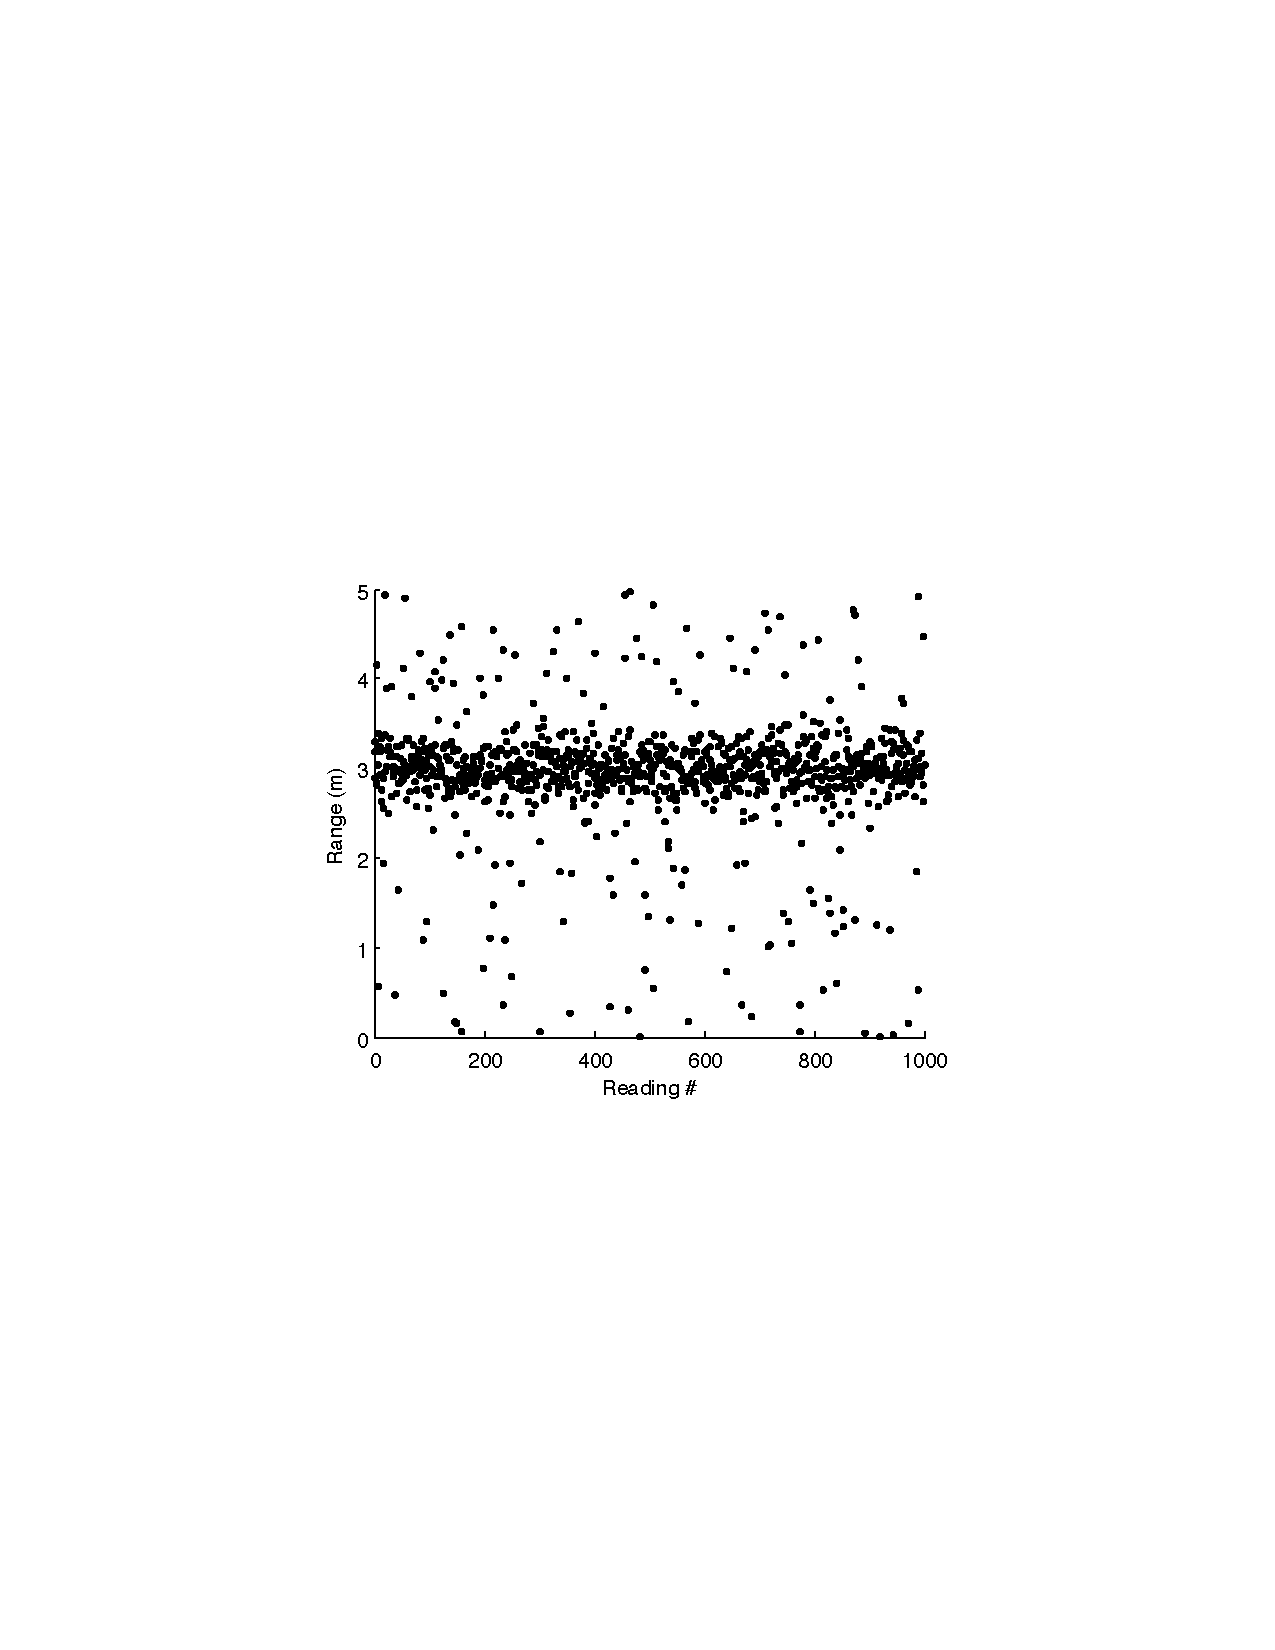
\includegraphics[scale=0.5]{images/range_readings}
  \caption{Range readings from sensor}
  \label{fig:range}
\end{figure}

If the sensor fails when obtaining a reading, it returns a value with
uniform probability in the range $[0,5]$. Otherwise, the sensor
returns a value distributed according to $N(\mu, \sigma^2)$, where
$\sigma^2$ is the variance of the sensor readings and $\mu$ is the
actual distance to the nearest obstacle. We will assume that
$\sigma^2$ is specified by the manufacturer of the sensor, and our
goal is to determine $\mu$ given a set of readings $x_1,\dots,x_n$.

The difficulty is that $\pi_0$, the failure rate of the sensor, is
unknown ahead of time, and we want to avoid biasing our estimate of
$\mu$ with completely meaningless samples where the sensor
failed. Therefore, we model a sensor reading $x_i$ according to the
outcome of a latent variable $z_i$ indicating whether or not the
sensor failed:
\begin{equation*}
  \label{eq:em-model}
  p(z_i = 0) = \pi_0,
  \qquad  p(x_i \mid z_i = 1) = \frac{1}{\sqrt{2\pi}\sigma} \exp \left\{ -\frac{1}{2\sigma^2}(x_i-\mu)^2 \right\},
  \qquad p(x_i \mid z_i = 0) = \frac{1}{5}\mathbf{1}(0\le x_{i}\le5)
\end{equation*}
This is a {\em mixture model} with two components: a Gaussian with
mean $\mu$ and variance $\sigma^2$, and a uniform over $[0,5]$.

%%%%%%%%%%%%%%%%%%%%%%%%%%%%%%%%%%%%%%%%%%%%%%%%%%%%%
\begin{enumerate}
\item \points{4} Using the equations defined above, write out the
  expression for the {\em marginal log likelihood} of a dataset $x_1,
  \dots, x_n$ given the parameters (this is what maximum likelihood is
  maximizing). Your solution should be in terms of $\pi_0, \sigma^2,
  \mu,$ and the $x_i$. {\em Hint: Remember to marginalize over the
    $z_i$'s.}  Write your final answer as: $\log p(x_1,\dots,x_n \mid
  \mu,\sigma^2,\pi_0) = \textrm{expression}$. Please show all your work/derivation for full credits.


%%%%%%%%%%%%%%%%%%%%%%%%%%%%%%%%%%%%%%%%%%%%%%%%%%%%%
\item \points{4} (E-Step) For fixed $\mu,\pi_0$, and $\sigma^2$,
  compute the posterior probabilities $q(z_i = 0 \mid x_i) = p(z_i = 0
  \mid x_, \mu,\pi_0,\sigma^2)$.  Hint: Remember $P(B \mid A) = P(A
  \mid B)P(B)/\sum_B P(A \mid B)P(B)$.  Your solution should be in
  terms of $\pi_0, \sigma^2, \mu,$ and the $x_i$.  Write your final
  answer as: $q(z_i = 0 \mid x_i) = \textrm{expression}$. Please show all your work/derivation for full credits.
  
  
%%%%%%%%%%%%%%%%%%%%%%%%%%%%%%%%%%%%%%%%%%%%%%%%%%%%%
\item \points{5} (M-step for $\mu$) Given the estimates of the
  posterior $q(z_i = 0 \mid x_i)$ and fixed $\pi_0$ and $\sigma^2$,
  now write down the update of $\mu$.  Your solution can include any
  of the following terms: $q(z_i = 0 \mid x_i), \pi_0, \sigma^2$ and
  the $x_i$.  Write your final answer as: $\mu = \textrm{expression}$. Please show all your work/derivation for full credits.


  
%%%%%%%%%%%%%%%%%%%%%%%%%%%%%%%%%%%%%%%%%%%%%%%%%%%%% 
\item \points{5} (M-step for $\pi_0$) Given the estimates of the
  posterior $q(z_i = 0 \mid x_i)$, updated $\mu$, and fixed
  $\sigma^2$, now write down the update for $\pi_0$.  Your solution
  can include any of the following terms: $q(z_i = 0 \mid x_i), \mu,
  \sigma^2$ and the $x_i$.  Write your final answer as: $\pi_0 =
  \textrm{expression}$. Please show all your work/derivation for full credits.
  

    
%%%%%%%%%%%%%%%%%%%%%%%%%%%%%%%%%%%%%%%%%%%%%%%%%%%%%
\item \points{5} Suppose we will now apply our EM procedure to the
  sample dataset in Figure$~\ref{fig:range}$. If we initialize $\mu = 0$ and $\pi_0 = 1/100$
  (with parameter $\sigma^2 = 1/2$) we get the following distribution
  for $q(z_i = 0 \mid x_i)$ as a function of the observation $x_i$:
  \begin{center}
    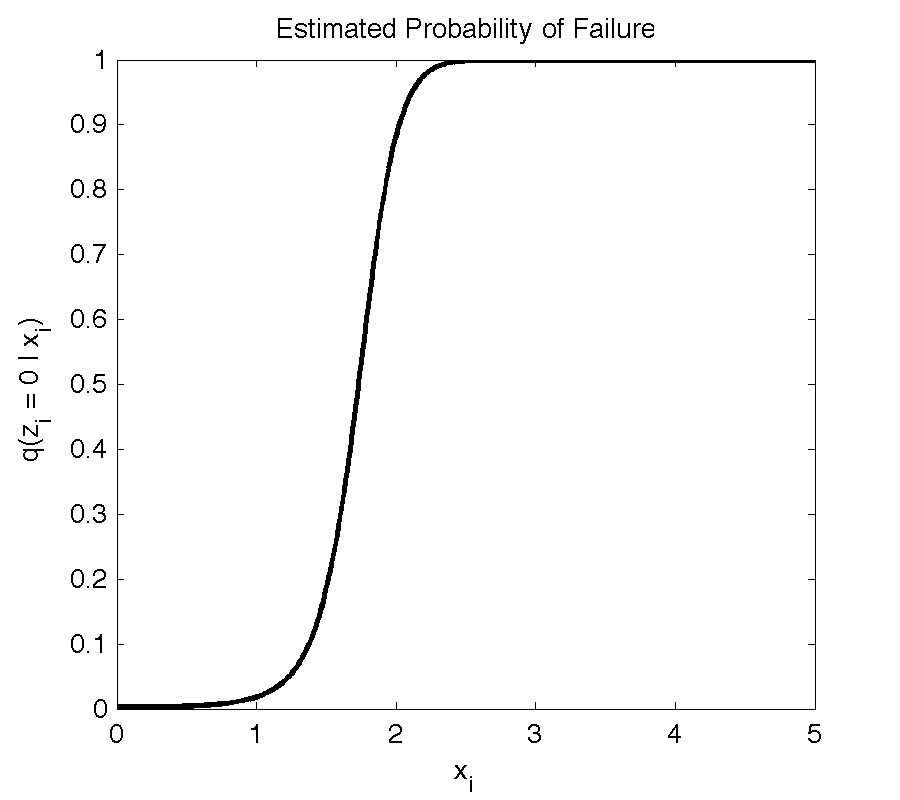
\includegraphics[width=0.4\textwidth]{images/q_mean0.png}
    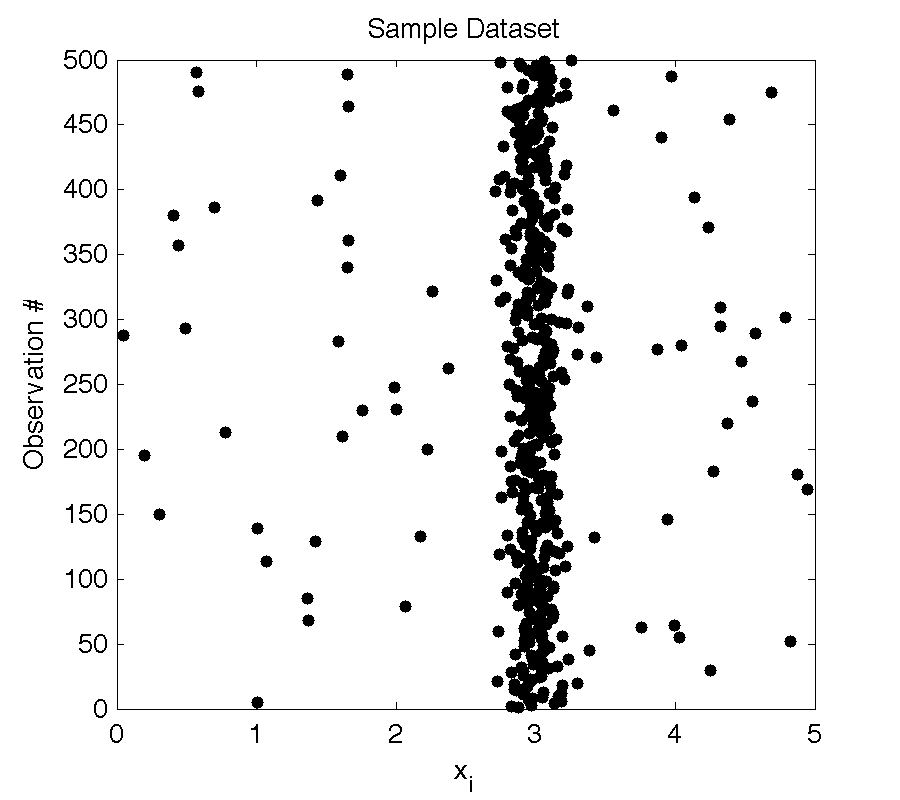
\includegraphics[width=0.4\textwidth]{images/range2.png}
  \end{center}
  Note that the plot of the data has been rotated to align with the
  plot of $q(z_i = 0 \mid x_i)$. 
  
  Will the EM algorithm converge to the correct $\mu$ value given this initialization?
  Briefly explain (2-3 sentences) your answer. Can you provide a better initialization in this situation?
  
  %Briefly explain (2-3 sentences) why we might expect this failure to
  %happen, given the above $q(z_i = 0 \mid x_i)$ distribution. 
  {\em Hint: Look at where the majority of points lie with respect to
    $q(z_i = 0 \mid x_i)$. How will this affect the update for $\pi_0$
    and $\mu$?}


\end{enumerate}
